\documentclass{article}\usepackage[]{graphicx}\usepackage[]{xcolor}
% maxwidth is the original width if it is less than linewidth
% otherwise use linewidth (to make sure the graphics do not exceed the margin)
\makeatletter
\def\maxwidth{ %
  \ifdim\Gin@nat@width>\linewidth
    \linewidth
  \else
    \Gin@nat@width
  \fi
}
\makeatother

\definecolor{fgcolor}{rgb}{0.345, 0.345, 0.345}
\newcommand{\hlnum}[1]{\textcolor[rgb]{0.686,0.059,0.569}{#1}}%
\newcommand{\hlsng}[1]{\textcolor[rgb]{0.192,0.494,0.8}{#1}}%
\newcommand{\hlcom}[1]{\textcolor[rgb]{0.678,0.584,0.686}{\textit{#1}}}%
\newcommand{\hlopt}[1]{\textcolor[rgb]{0,0,0}{#1}}%
\newcommand{\hldef}[1]{\textcolor[rgb]{0.345,0.345,0.345}{#1}}%
\newcommand{\hlkwa}[1]{\textcolor[rgb]{0.161,0.373,0.58}{\textbf{#1}}}%
\newcommand{\hlkwb}[1]{\textcolor[rgb]{0.69,0.353,0.396}{#1}}%
\newcommand{\hlkwc}[1]{\textcolor[rgb]{0.333,0.667,0.333}{#1}}%
\newcommand{\hlkwd}[1]{\textcolor[rgb]{0.737,0.353,0.396}{\textbf{#1}}}%
\let\hlipl\hlkwb

\usepackage{framed}
\makeatletter
\newenvironment{kframe}{%
 \def\at@end@of@kframe{}%
 \ifinner\ifhmode%
  \def\at@end@of@kframe{\end{minipage}}%
  \begin{minipage}{\columnwidth}%
 \fi\fi%
 \def\FrameCommand##1{\hskip\@totalleftmargin \hskip-\fboxsep
 \colorbox{shadecolor}{##1}\hskip-\fboxsep
     % There is no \\@totalrightmargin, so:
     \hskip-\linewidth \hskip-\@totalleftmargin \hskip\columnwidth}%
 \MakeFramed {\advance\hsize-\width
   \@totalleftmargin\z@ \linewidth\hsize
   \@setminipage}}%
 {\par\unskip\endMakeFramed%
 \at@end@of@kframe}
\makeatother

\definecolor{shadecolor}{rgb}{.97, .97, .97}
\definecolor{messagecolor}{rgb}{0, 0, 0}
\definecolor{warningcolor}{rgb}{1, 0, 1}
\definecolor{errorcolor}{rgb}{1, 0, 0}
\newenvironment{knitrout}{}{} % an empty environment to be redefined in TeX

\usepackage{alltt}
\usepackage{amsmath} %This allows me to use the align functionality.
                     %If you find yourself trying to replicate
                     %something you found online, ensure you're
                     %loading the necessary packages!
\usepackage{amsfonts}%Math font
\usepackage{graphicx}%For including graphics
\usepackage{hyperref}%For Hyperlinks
\usepackage[shortlabels]{enumitem}% For enumerated lists with labels specified
                                  % We had to run tlmgr_install("enumitem") in R
\hypersetup{colorlinks = true,citecolor=black} %set citations to have black (not green) color
\usepackage{natbib}        %For the bibliography
\setlength{\bibsep}{0pt plus 0.3ex}
\bibliographystyle{apalike}%For the bibliography
\usepackage[margin=0.50in]{geometry}
\usepackage{float}
\usepackage{multicol}

%fix for figures
\usepackage{caption}
\newenvironment{Figure}
  {\par\medskip\noindent\minipage{\linewidth}}
  {\endminipage\par\medskip}
\IfFileExists{upquote.sty}{\usepackage{upquote}}{}
\begin{document}

\vspace{-1in}
\title{Lab 7 and 8 -- MATH 240 -- Computational Statistics}

\author{
  Caroline Devine \\
  Colgate University  \\
  Math Department  \\
  {\tt cdevine@colgate.edu}
}

\date{April 1st, 2025}

\maketitle

\begin{multicols}{2}
\begin{abstract}
This document provides a basic template for the 2-page labs we will complete each week. Here, briefly summarize what you did and why it might be helpful. Provide all the top-line conclusions, but avoid providing \emph{all} the details. Results should be limited to ``we show X, Y, and Z."
\end{abstract}

\noindent \textbf{Keywords:} What topics does the lab cover concerning class? List 3-4 key terms here, separated by semicolons.

\section{Introduction}



\section{Density Functions and Parameters}
\textbf{ADD PDF of beta}
\textbf{ADD parameters}

To explore the beta distribution, we focused on four cases: \(\text{Beta}(\alpha = 2, \beta = 5)\), \(\text{Beta}(\alpha = 5, \beta = 5)\), \(\text{Beta}(\alpha = 5, \beta = 2)\), and \(\text{Beta}(\alpha = 0.5, \beta = 0.5)\). We calculated the population-level characteristics(mean, variance, skewness, and excess kurtosis) for all four cases by deriving the formulas and numerically analyzing them for each case (Summarized in Table 1). 



% latex table generated in R 4.4.2 by xtable 1.8-4 package
% Mon Mar 31 17:27:25 2025
\begin{table}[H]
\centering
\begingroup\small
\begin{tabular}{rrrrrr}
  \hline
Alpha & Beta & mean & variance & skewness & kurtosis \\ 
  \hline
2.00 & 5.00 & 0.29 & 0.03 & 0.60 & -0.12 \\ 
  5.00 & 5.00 & 0.50 & 0.02 & 0.00 & -0.46 \\ 
  5.00 & 2.00 & 0.71 & 0.03 & -0.60 & -0.12 \\ 
  0.50 & 0.50 & 0.50 & 0.12 & 0.00 & -1.50 \\ 
   \hline
\end{tabular}
\endgroup
\caption{Population-Level Summary by Case} 
\label{Table 1}
\end{table}

To visually see the distribution, all four cases are plotted in Figure 1. The \(\text{Beta}(\alpha = 2, \beta = 5)\) distribution is right-skewed, the \(\text{Beta}(\alpha = 5, \beta = 5)\) is symmetric, the \(\text{Beta}(\alpha = 5, \beta = 2)\) is left-skewed, and the \(\text{Beta}(\alpha = 0.5, \beta = 0.5)\) is u-shaped indicating majority of the distribution is close to 0 or 1. We can see from Figure 1 that when \(\alpha\) \(<\) \(\beta\), it is right-skewed; when \(\alpha\) \(>\) \(\beta\), it is left-skewed; when \(\alpha\)  = \(\beta\), it is symmetric. 

\section{Properties}
The beta distribution includes many important properties such as mean, variance, skewness, and excess kurtosis. These values were calculated for all four cases using provided formulas from beta distribution (Table \ref{Table 1}). To compare the results, the moments of the beta distribution were calculated directly using numerical integration. Our function, \texttt{beta.moment()}, calculated both the centered and uncentered moments, summarizing the same characteristics as in Table \ref{Table 1}. This process resulted in values that match the theoretical values from Table \ref{Table 1} and can be seen in Table \ref{Table 2} in Appendix. 

Since the goal of summarizing this data is to approximate what the population distribution might be, we further analyze how different sample sizes effect the sample estimates. Initially randomly selecting sample sizes of \texttt{n} = 500 from the beta distribution, histograms for each sample with estimated density and true PDF were plotted (Figure \ref{plot2}) accompanied by a numerical summary (Table \ref{Table 3}). Comparing numerical summaries and plots from sample to Table \ref{Table 1}, confirms that the sample estimates the approximate theoretical values. 

\section{Estimators}

\section{Example}

\section{Discussion}


%%%%%%%%%%%%%%%%%%%%%%%%%%%%%%%%%%%%%%%%%%%%%%%%%%%%%%%%%%%%%%%%%%%%%%%%%%%%%%%%
% Bibliography
%%%%%%%%%%%%%%%%%%%%%%%%%%%%%%%%%%%%%%%%%%%%%%%%%%%%%%%%%%%%%%%%%%%%%%%%%%%%%%%%
\vspace{2em}

\noindent\textbf{Bibliography:} Note that when you add citations to your bib.bib file \emph{and}
you cite them in your document, the bibliography section will automatically populate here.

\begin{tiny}
\bibliography{bib}
\end{tiny}
\end{multicols}

%%%%%%%%%%%%%%%%%%%%%%%%%%%%%%%%%%%%%%%%%%%%%%%%%%%%%%%%%%%%%%%%%%%%%%%%%%%%%%%%
% Appendix
%%%%%%%%%%%%%%%%%%%%%%%%%%%%%%%%%%%%%%%%%%%%%%%%%%%%%%%%%%%%%%%%%%%%%%%%%%%%%%%%
\newpage
\onecolumn
\section{Appendix}

\begin{figure}[H]
\begin{center}
\begin{knitrout}
\definecolor{shadecolor}{rgb}{0.969, 0.969, 0.969}\color{fgcolor}
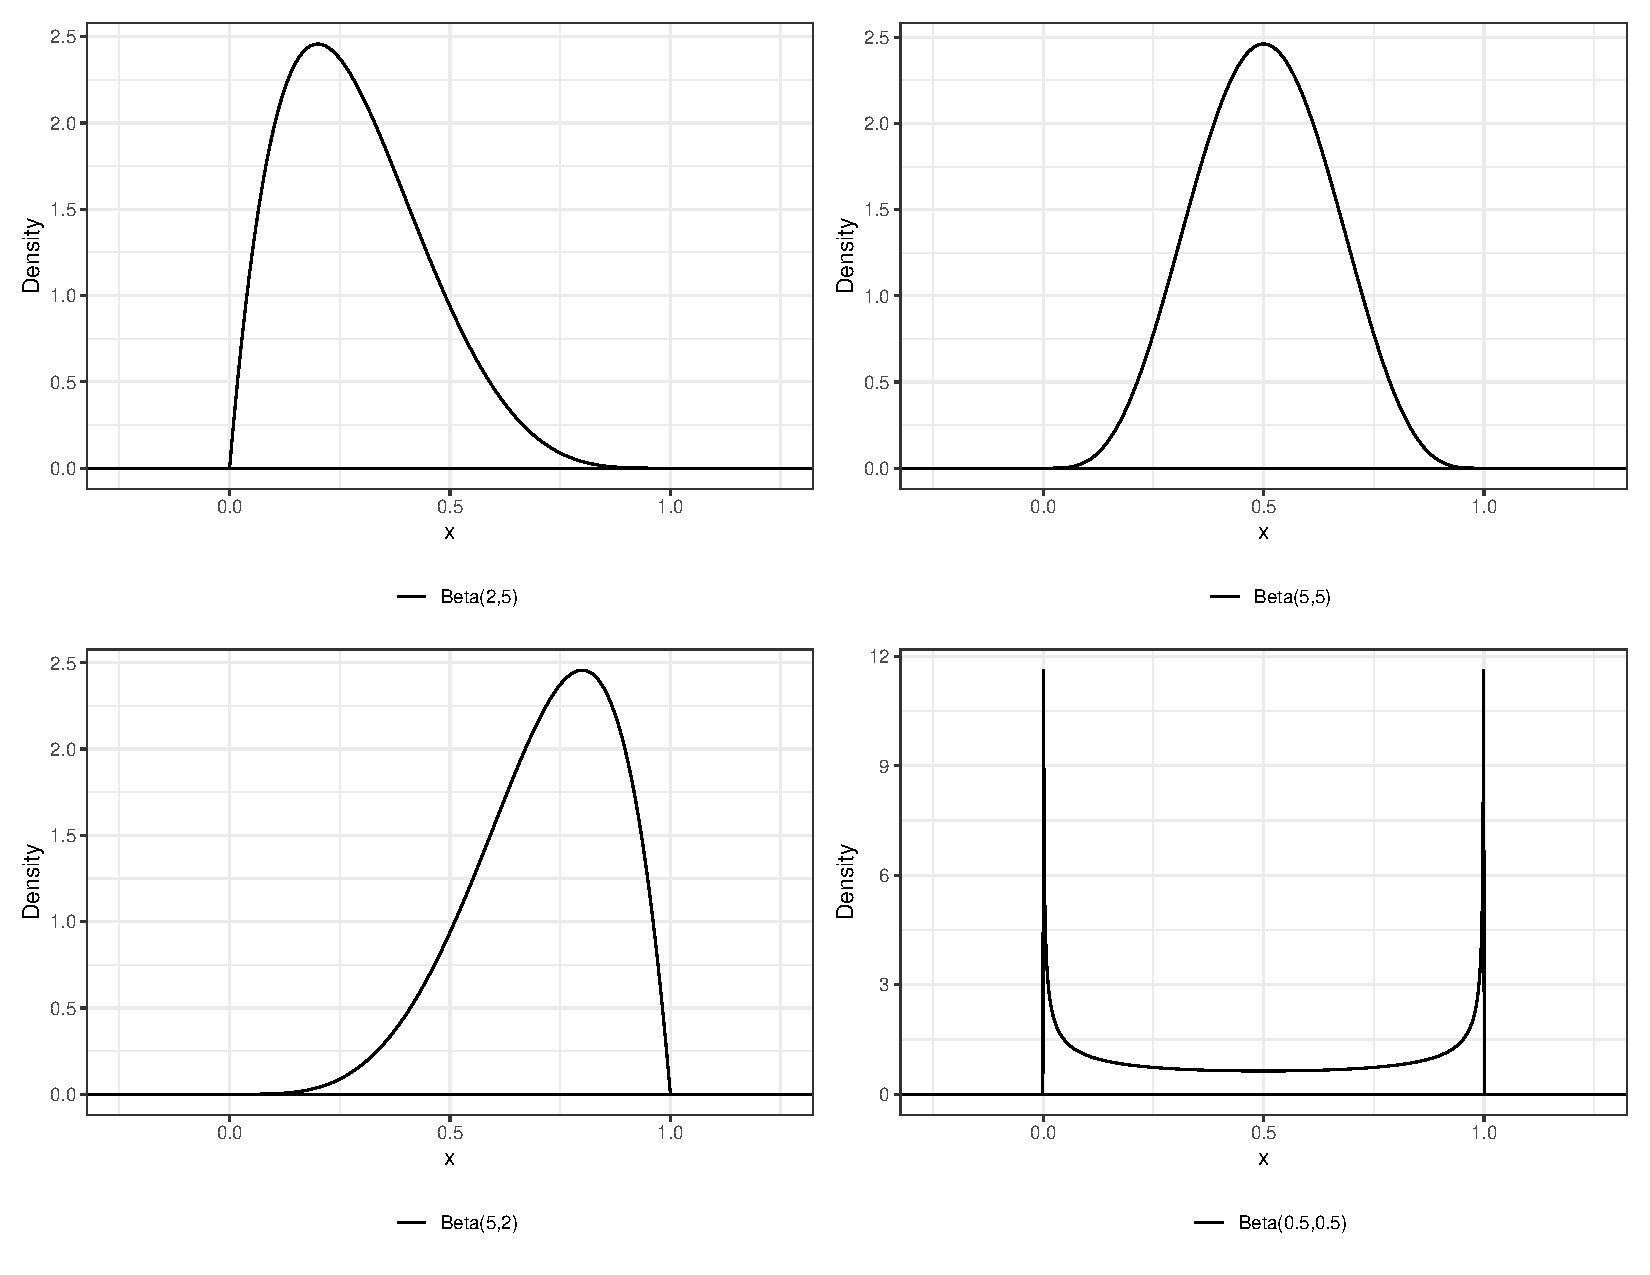
\includegraphics[width=\maxwidth]{figure/unnamed-chunk-3-1} 
\end{knitrout}
\caption{Population Distribution Plot by Case}
\label{plot1} 
\end{center}
\end{figure}




% latex table generated in R 4.4.2 by xtable 1.8-4 package
% Mon Mar 31 17:27:25 2025
\begin{table}[H]
\centering
\begingroup\small
\begin{tabular}{rrrrrr}
  \hline
Alpha & Beta & mean & variance & skewness & excess.kurtosis \\ 
  \hline
2.00 & 5.00 & 0.29 & 0.03 & 0.60 & -0.12 \\ 
  5.00 & 5.00 & 0.50 & 0.02 & -0.00 & -0.46 \\ 
  5.00 & 2.00 & 0.71 & 0.03 & -0.60 & -0.12 \\ 
  0.50 & 0.50 & 0.50 & 0.12 & -0.00 & -1.50 \\ 
   \hline
\end{tabular}
\endgroup
\caption{Moments Summary Table} 
\label{Table 2}
\end{table}



\begin{figure}[H]
\begin{center}
\begin{knitrout}
\definecolor{shadecolor}{rgb}{0.969, 0.969, 0.969}\color{fgcolor}

{\centering 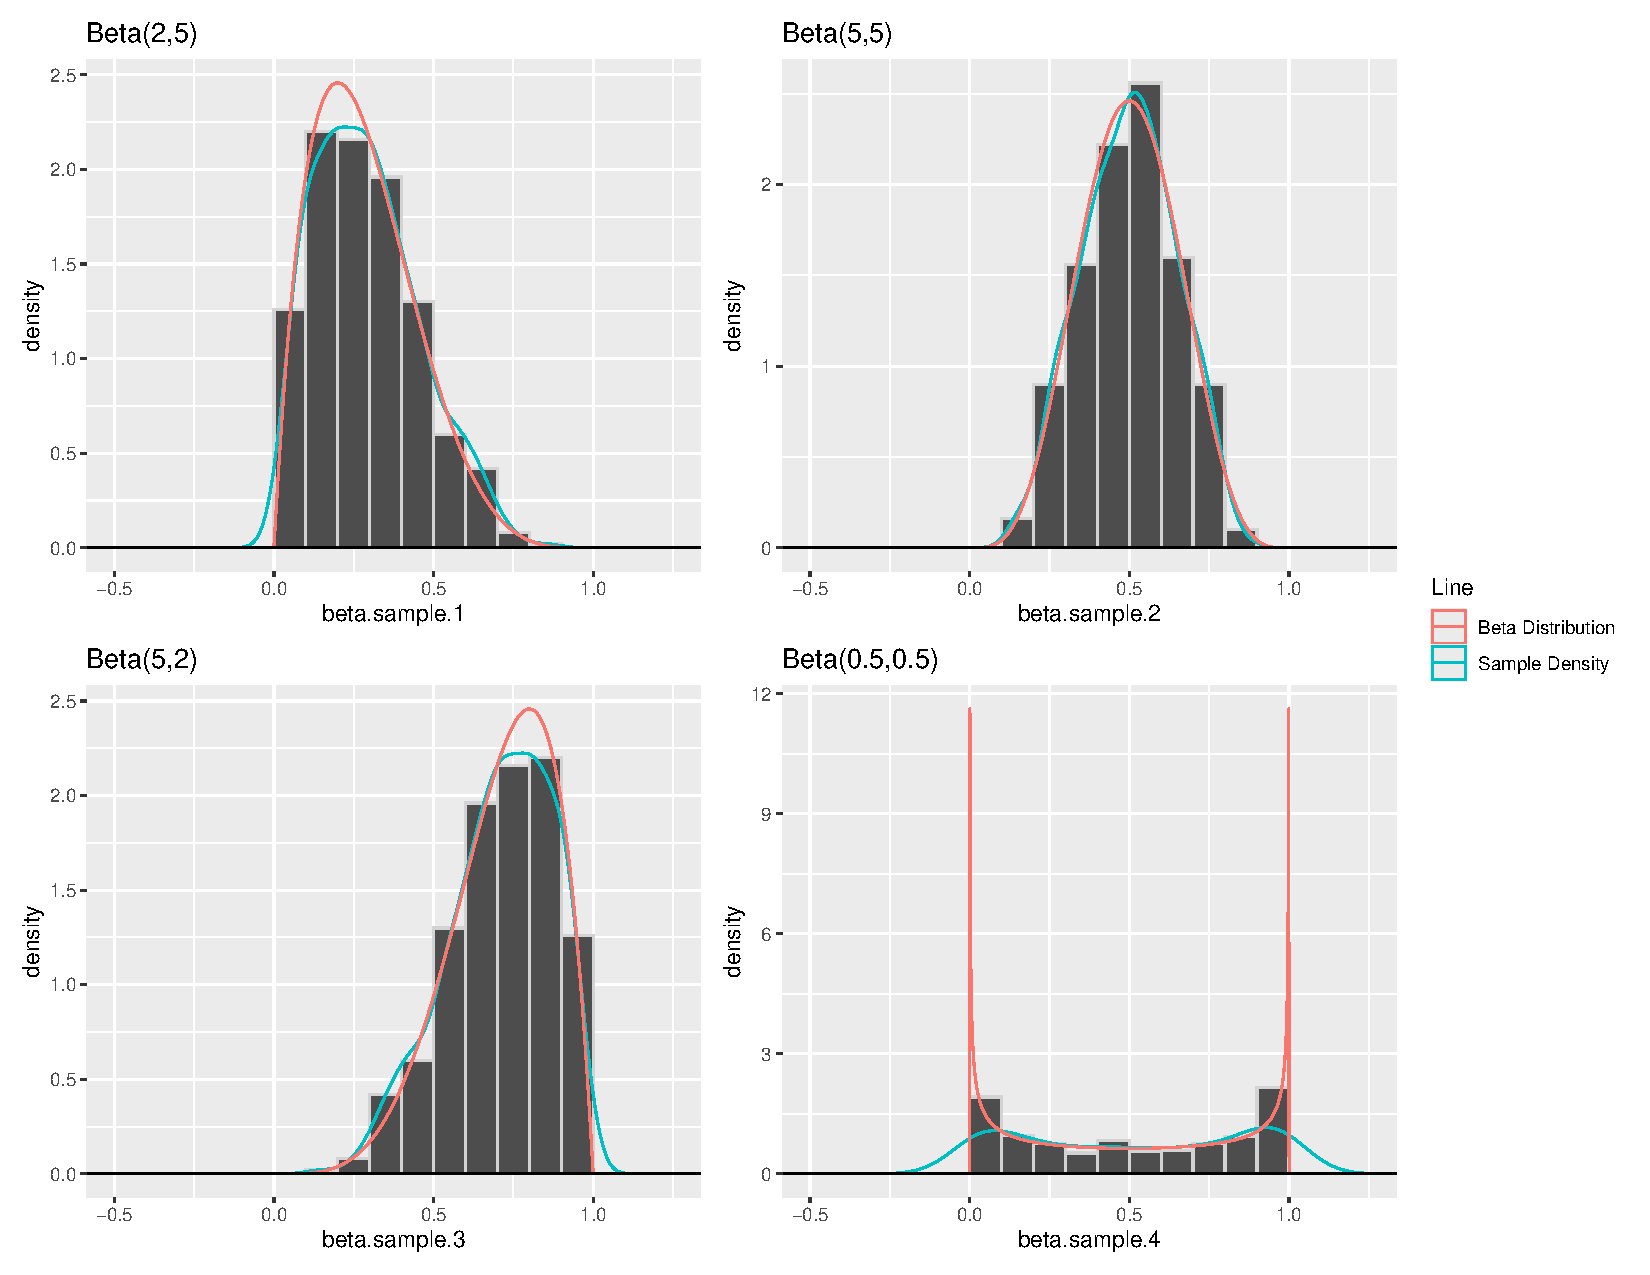
\includegraphics[width=\maxwidth]{figure/unnamed-chunk-6-1} 

}


\end{knitrout}
\caption{Sample Plot by Four Beta Distributions}
\label{plot2} 
\end{center}
\end{figure}

% latex table generated in R 4.4.2 by xtable 1.8-4 package
% Mon Mar 31 17:27:25 2025
\begin{table}[H]
\centering
\begingroup\small
\begin{tabular}{rrrrrr}
  \hline
Alpha & Beta & mean & variance & skewness & excess.kurtosis \\ 
  \hline
2.00 & 5.00 & 0.29 & 0.03 & 0.60 & -0.12 \\ 
  5.00 & 5.00 & 0.50 & 0.02 & -0.00 & -0.46 \\ 
  5.00 & 2.00 & 0.71 & 0.03 & -0.60 & -0.12 \\ 
  0.50 & 0.50 & 0.50 & 0.12 & -0.00 & -1.50 \\ 
   \hline
\end{tabular}
\endgroup
\caption{Sample Summary Table} 
\label{Table 3}
\end{table}


\end{document}
